\subsection{Padding}
\begin{frame}{}
    \LARGE CNN Hyperparameter: \textbf{Padding}
\end{frame}

\begin{frame}[allowframebreaks]{Padding}
\begin{itemize}
    \item Applying Convolution as such reduces the size of the borders.
    \item Sometimes this is not desirable.
    \item We can pad the border with zeros.
\end{itemize}


\begin{figure}
\centering
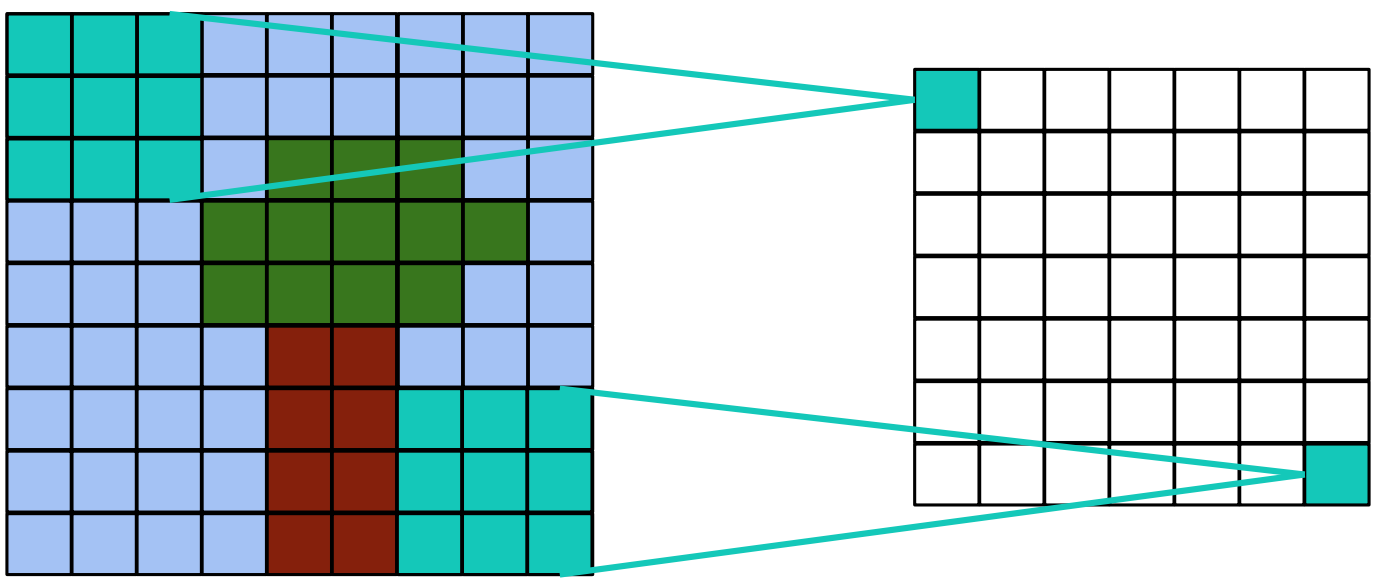
\includegraphics[width=1.0\textwidth,height=0.7\textheight,keepaspectratio]{images/cnn/pad_1.png}
\end{figure}

\framebreak

\begin{itemize}
    \item Same Convolution: Output is the same size as input
\end{itemize}


\begin{figure}
\centering
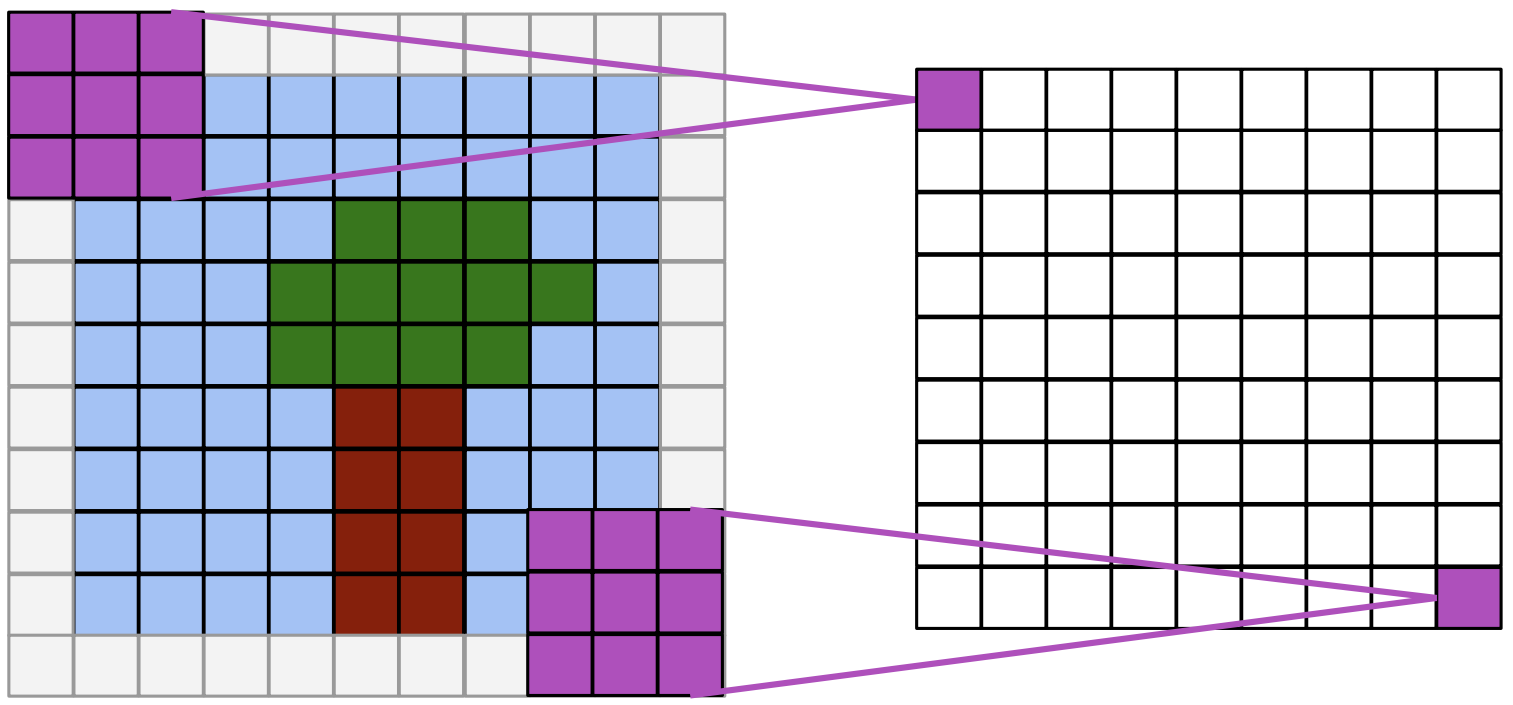
\includegraphics[width=1.0\textwidth,height=0.8\textheight,keepaspectratio]{images/cnn/pad_3.png}
\end{figure}


\framebreak

\begin{itemize}
    \item Full Convolution: output size = input size + kernel size - 1
\end{itemize}


\begin{figure}
\centering
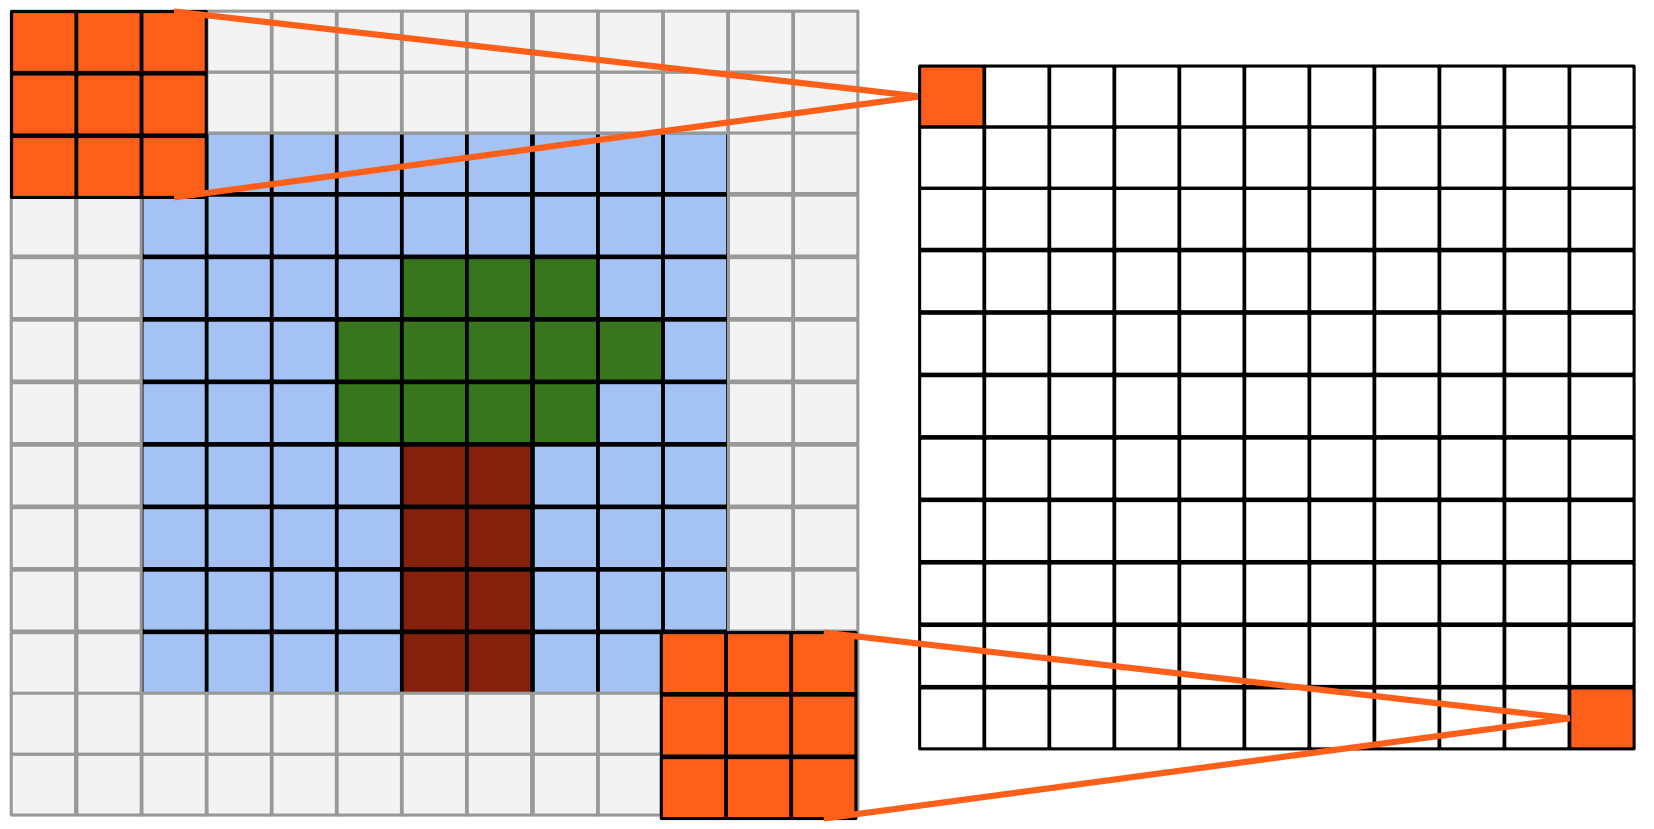
\includegraphics[width=1.0\textwidth,height=0.8\textheight,keepaspectratio]{images/cnn/pad_2.png}
\end{figure}
    
\end{frame}